\begin{figure}[h!]
\begin{center}
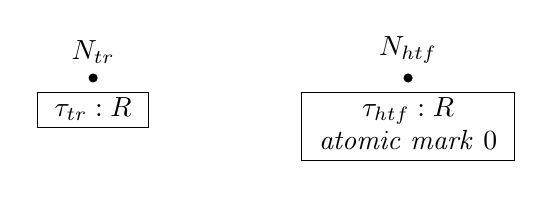
\begin{tikzpicture}[yscale=-1,
place/.style={circle,draw=black, fill=black, inner sep=0pt, 
              minimum size=1mm}]

 \node[place] (1st) at (1, 0) [label=above: $N_{tr}$,
                               label=below: 
            \begin{tabular}{|l|}
             \hline
             $\tau_{tr} : R$\\
             \hline
            \end{tabular}
] {};
	

\begin{scope}[xshift=4cm]
  \node[place] (1st) at (1, 0) [label=above: $N_{htf}$,
                               label=below: 
            \begin{tabular}{|c|}
              \hline
              $\tau_{htf} : R$\\
              \textit{atomic mark} 0\\
              \hline
            \end{tabular}] {};
\end{scope}


\end{tikzpicture}
\end{center}
\caption{Similarity between tr and htf}
\label{fig:SimTrHtf}
\end{figure}